% ****** Start of file apssamp.tex ******
%
%   This file is part of the APS files in the REVTeX 4.2 distribution.
%   Version 4.2a of REVTeX, December 2014
%
%   Copyright (c) 2014 The American Physical Society.
%
%   See the REVTeX 4 README file for restrictions and more information.
%
% TeX'ing this file requires that you have AMS-LaTeX 2.0 installed
% as well as the rest of the prerequisites for REVTeX 4.2
%
% See the REVTeX 4 README file
% It also requires running BibTeX. The commands are as follows:
%
%  1)  latex apssamp.tex
%  2)  bibtex apssamp
%  3)  latex apssamp.tex
%  4)  latex apssamp.tex
%
\documentclass[%
 reprint,
%superscriptaddress,
%groupedaddress,
%unsortedaddress,
%runinaddress,
%frontmatterverbose, 
%preprint,
%preprintnumbers,
%nofootinbib,
%nobibnotes,
%bibnotes,
 amsmath,amssymb,
 aps,
%pra,
%prb,
%rmp,
%prstab,
%prstper,
%floatfix,
]{revtex4-2}

\usepackage{graphicx}% Include figure files
\usepackage{dcolumn}% Align table columns on decimal point
\usepackage{bm}% bold math
\usepackage{hyperref}% add hypertext capabilities
\usepackage[mathlines]{lineno}% Enable numbering of text and display math
%\linenumbers\relax % Commence numbering lines
\newcommand{\sgn}{\text{sgn}}
\usepackage [english]{babel}
\usepackage [autostyle, english = american]{csquotes}
\MakeOuterQuote{"}
\usepackage{indentfirst}
\usepackage{subcaption}


%\usepackage[showframe,%Uncomment any one of the following lines to test 
%%scale=0.7, marginratio={1:1, 2:3}, ignoreall,% default settings
%%text={7in,10in},centering,
%%margin=1.5in,
%%total={6.5in,8.75in}, top=1.2in, left=0.9in, includefoot,
%%height=10in,a5paper,hmargin={3cm,0.8in},
%]{geometry}

\begin{document}

\preprint{APS/123-QED}

\title{Statistical Mechanics of Recurrent Neural Networks Based on Physical Models}% Force line breaks with \\
% \thanks{A footnote to the article title}%

\author{Qu Yuxuan}
 % \altaffiliation[Also at ]{Physics Department, XYZ University.}%Lines break automatically or can be forced with \\
\email{quyu0001@e.ntu.edu.sg}
\author{Lucas Seah}%
 \email{seah0222@e.ntu.edu.sg}
\affiliation{%
 NTU
}%

% \collaboration{MUSO Collaboration}%\noaffiliation

% \author{Charlie Author}
%  \homepage{http://www.Second.institution.edu/~Charlie.Author}
% \affiliation{
%  Second institution and/or address\\
%  This line break forced% with \\
% }%
% \affiliation{
%  Third institution, the second for Charlie Author
% }%
% \author{Delta Author}
% \affiliation{%
%  Authors' institution and/or address\\
%  This line break forced with \textbackslash\textbackslash
% }%

% \collaboration{CLEO Collaboration}%\noaffiliation

\date{\today}% It is always \today, today,
             %  but any date may be explicitly specified

\begin{abstract}
The Ising model was identified to be the first recurrent neural network. In this paper, we try to explain what the statement means, hence reviewing how the inverse Ising problem is unsupervised learning, and how statistical mechanics can be used to analyze the behaviour of a restricted Boltzmann machine with binary weights, yielding phase transitions.
% \begin{description}
% \item[Usage]
% Secondary publications and information retrieval purposes.
% \item[Structure]
% You may use the \texttt{description} environment to structure your abstract;
% use the optional argument of the \verb+\item+ command to give the category of each item. 
% \item[Keywords] Belief Propagation, Bethe Approximation, Cavity Method, Inverse Ising Problem, Phase Transition, Recurrent Neural Network, Restricted Boltzmann Machine
% \end{description}
\end{abstract}

%\keywords{Suggested keywords}%Use showkeys class option if keyword
                              %display desired
\maketitle

%\tableofcontents

\section{\label{sec:level1}Introduction}

The proliferation of Artificial Neural Networks, Artificial Intelligence and Machine Learning have seen a rise in research and development in this area. Its usefulness and applicability span a myriad of sectors including analytical chemistry \cite{DEBUS2021116459}, drug discovery and development \cite{jimenez2020drug}, particle physics \cite{Shlomi_2021}, astrophysics \cite{george2018deep}, and understanding our brain. While its development has come a long way to advanced algorithms and robust infrastructures, it is interesting to study its genesis and its close ties with statistical mechanics.


\section{\label{sec:NN for ML}Neural Networks for Machine Learning}
% \section{Neural Networks, Machine Learning and Similarities in Statistical Mechanics}
% This section seeks to understand what neural networks and machine learning are and how do they tie in with statistical mechanics. Information about neural networks and how they learn through machine learning will also be introduced briefly, providing sufficient detail for discussions related to statistical mechanics. We will be discussing what does it mean for a neural network to learn and the several techniques employed in machine learning. A summary and the mathematical framework for neural networks will be established to provide the reader sufficient knowledge to understand the project. We will introduce the connections between neural network and machine learning to statistical mechanics and in a later section, draw the link from the Ising model to Recurrent Neural Network.

% \subsection{Neural Networks}
Neural networks are inspired by the structure and function neural circuits in the human brain \cite{rumelhart1986parallel} \cite{charu2018neural}. A typical feedforward neural networks (FNN) can be modeled by weighted, directed graphs (the mathematical object). Nodes (neurons) are organised into three layers - input, hidden, and output. The links (synapses) which have weights that determine the strength of interaction betwen nodes and impact information processing. Data points are fed into input nodes of the network. Neuron activation values of layers are calculated from the preceding layers through the weights, which are represented by a feature matrix and the activation function. The processed information is fed forward through the network, producing an output\cite{goodfellow2016deep}.

% \subsection{Machine Learning}
Machine learning employs algorithms and statistical models to computer programs on a data set to learn patterns and make predictions about the data set. There are several approach to machine learning --- supervised learning, unsupervised learning, reinforcement learning. We're primarily focused on unsupervised learning. It is learning from unlabeled data, finding patterns or underlying structures within the data \cite{murphy2012machine}.

A type of neural network we are interested in are recurrent neural networks (RNN). Unlike FNNs, RNNs are bidirectional which can be represented by an undirected graph. This means that output from some nodes are able to affect subsequent input to the same nodes \cite{dupond2019thorough}\cite{tealab2018time}. In particular, we are interested in a type of unsupervised learning that is called auto-associative self-supervised feature learning. What it does is that a neural network is trained on its own output data after forgetting its original feature matrix used to generate those data, so as to reconstruct the feature matrix and reproduce the same output data statistics \cite{kramer1991nonlinear}. This is the fundamental task of neural networks known as auto-encoders \cite{SCHNEIDER2022149}. 
% As such, we are then able to use multiple samples of outputs generated from the teacher model. Without the student model knowing what the teacher model is and only from the generated outputs of the teacher model, the student model will reconstruct the true feature vector of the teacher model.

% \subsection{Connection to Statistical Mechanics}
% To understand the link between statistical mechanics and neural network, we first need to look at an problem inspiring the use of statistical physics. The K-SAT problem is finding a solution of N Boolean variables to satisfy a random composition of logical AND inside M clauses. Each clause is satisfied as logical OR of K randomly selected distinct variables \cite{huang2021statistical_msim}. For instance:
% \begin{align}
%     \mathcal{F} = (\bar{x_2}\land x_4)\lor(x_3\land\bar{x_1} )
% \end{align}
% This is akin to the spin glass problem. If $x_i$ is TRUE, then we can take the Ising spin to be an up spin (+1), likewise if $x_i$ is FALSE, then we can take the Ising spin to be a down spin (-1). In statistical physics, an energy function incorporates the concept of "violated clauses" from conditions akin to those found in the K-SAT problem to the context of spin configurations. In this scenario, these "violated clauses" specifically denote instances where the arrangement of spins doesn't comply with constraints, similar to logical constraints encountered in the K-SAT problem. Thus, the energy function can be determined by the count of violated clauses when provided with a spin configuration as such:
% \begin{align}
%     H(\boldsymbol{\sigma})=\sum_{m=1}^M \prod^K_{j=1} \frac{1+J_j^m \sigma_{i^m_j}}{2}
% \end{align}

% With the activation function as the energy function, the number of violated clauses reflects how well the spin arrangement aligns or deviates from the prescribed rules or conditions. This is similar to the satisfaction or violation of clauses in the K-SAT problem.\\
% In the mean field limit, where the number of Boolean variables and number of clauses approach infinity while keeping the ratio constant $N\to\infty,M\to\infty \space$ s.t. $\frac{M}{N} = c$, interesting phase transition occur.\\
% The Ising model was found to be a recurrent neural network that was able to learn \cite{amari1972learning}\cite{amari1972characteristics}\cite{doi:10.1073/pnas.79.8.2554}. As such, we are able to use RBM and use statistical mechanics techniques to study phase transitions in neural networks like RBM. In this paper, we will thus investigate at these phase transition, what does it mean for an Ising model to learn and does the "temperature" of the data set affect the learning capabilities for the Ising model.


\section{Ising Model as an RNN for Unsupervised Learning}
In this section, we introduce the Ising problem for spin glass models, summarize and discuss some techniques to solve the Ising problem, and explain why the Ising/spin glass models can be considered RNNs. Then, we introduce the inverse Ising problem and explain how it is essentially unsupervised learning. 

\subsection{The Ising problem of Spin Glass Models}
The original Ising problem \cite{yeomans1992statistical} was a problem in many body physics entailing the solution of the magnetization (per spin), $m$, of a lattice of $N$ spins, each admitting values -1 and 1, given that neighbouring spins interact with the same coupling constants, $J$, every spin experiences an external magnetic field $H$ and the system has an inverse temperature $\beta$.

If we view the spins as neurons, magnetization of each spin as neuron activation values, and $J$ as the weights of the synapses between the neurons, and let $H=0$, then there is a close correspondence between the Ising model and the neural network. Crucially, it is the fact that the Ising model reaches equilibrium given $J$ and $\beta$ which allows the calculation of magnetization \cite{schmidhuber2022annotated}. However, if there is only a single $J$ for all the synapses, all neurons end up with the same magnetization, and it would not be a really useful neural network. Therefore, spin glass models are needed to capture the complexity of neural networks. 

We introduce the general spin model \cite{huang2021statistical_cavity} by comparing its Hamiltonian (Equation \ref{eq:spinglass_H}) with that of the original Ising model (Equation \ref{eq:ising_H}) in the absence of an external field. 
\begin{align}
    \mathcal{H}&=-\frac{1}{2}\sum_i\sum_{j \in \partial i} J s_i s_j \label{eq:ising_H} \\
    \mathcal{H}&=-\sum_{a} J_{a} \prod_{i=1}^N s_i\label{eq:spinglass_H}
\end{align}
Note that $\partial i$ is the set of indices of spins that are immediate neighbours of spin $i$. 
The general spin glass Hamiltonian is highly complex. There can be arbitrarily many interactions between spins up to all spins in the spin glass. If only unique pair-wise interactions are allowed, then the spin glass model fits the description of a general RNN (with no hidden nodes). If we further restrict the model to nearest neighbour interactions only, then the original Ising model is recovered.

\subsection{Solving the Ising Problem of Spin Glass Models}

There are various ways to solve the spin glass model. We look at two methods.

% The TAP equations are derived with the high temperature series expansion which can also used to solve the original Ising model \cite{huang2021statistical_TAP}.

% The replica method is essentially a clever mathematical trick that simplifies the calculation. 
% The calculations can get very involved, so we will not describe how the magnetization of the $i$-th spin is calculated with the replica method.
% Nonetheless, it involves interesting concepts from spin glass physics. 
The replica method uses the important property \cite{huang2021statistical_self_avg} originating from spin glass physics that the free energy of the spin glass due to \textit{a particular realization} of $\{J_{ij}\}$ converges quickly to the quenched average free energy $\langle - (\ln{Z})/\beta \rangle_d$ in the thermodynamic limit ($N \rightarrow \infty$). Note that $Z$ is the partition function while the $\langle \bullet \rangle_d$, known as the disorder average, is the average over \textit{all possible realizations} of $\{J_{ij}\}$. Unfortunately, the quenched average free energy is notoriously difficult to calculate, hence the replica trick is needed. It can be shown \cite{huang2021statistical_replica_trick} that 
\begin{equation}
    \lim_{N\rightarrow \infty} \frac{\langle \ln{Z} \rangle_d}{N\beta}  = \lim_{n\rightarrow 0} \lim_{N\rightarrow \infty} \frac{\ln{\langle Z^n \rangle_d}}{nN\beta} \label{eq:replica_trick}
\end{equation}
In the literature, $(\ln{\langle Z^n \rangle})/\beta$ is known as the annealed average free energy of a composite system consisting of $n$ replicas of the original system, hence the name "replica method". The quenched and annealed averages describe very different physical pictures \cite{Castellani_2005}. The quenched average is an average of free energy over all the realizations of $\{J_{ij}\}$, but the annealed average treats each $J_{ij}$ to be fluctuating just like each spin value. Then, it can be shown \cite{huang2021statistical_replica_F} that the free energy is a function of many order parameters:
\begin{equation}
    F=F\left( (r_{\rho \sigma})_{(\rho,\sigma)=(1,1)}^{(n,n)}, (\hat{q}_{\rho \sigma})_{(\rho,\sigma)=(1,1)}^{(n,n)}, (m_\rho)_{\rho=1}^{n} \right) \label{eq:replica_F}
\end{equation}
where $\rho, \sigma$ are indices over the replica systems. The first order approximation is always obtained through the replica symmetric ansatz \cite{huang2021statistical_replica_sym}, which assume that the order parameters are the same over all indices such that there are only three order parameters $\hat{q},r,m$. Such solutions can become unstable or unphysical when the temperature is low. In such a case, there has to be replica symmetry breaking \cite{huang2021statistical_replica_sym_break} in the free energy expression, yielding higher order approximations. However, the reason why the replica trick works is enigmatic. There is no clear physical intuition behind it, and neither is its mathematical derivation truly rigorous \cite{huang2021statistical_replica_trick}. 

The cavity method \cite{huang2021statistical_cavity}, equivalent to the variational Bethe approximation from Physics and belief propagation from Computer Science \cite{huang2021statistical_Bethe}, solves the magnetization from a self-consistent equation through iterations of the so-called message passing equations. The cavity method is formalized over factor graph representations of the problem. 

Firstly, notice that the partition function of the spin glasses can be written as
\begin{equation}
\begin{split}
            Z 
        &= \sum_{\{ s_i \}_{i=1}^N}\exp{\left( -\sum_{a} J_{a} \prod_{i=1}^N s_i \right)}\\ 
        &= \sum_{\{ s_i \}_{i=1}^N}\prod_{a} \exp{\left(- J_{a} \prod_{i=1}^N s_i \right)}
\end{split}
    \label{eq:spinglass_Z}
\end{equation}
A factor graph is a representation for the product of functions. Each function is represented by a square node or the so-called a factor node. All variables are represented by circular nodes or the so-called variable nodes. If a function takes a variable as an input, there is an unweighted link between the corresponding factor node and variable node. Therefore, the factor graph of spin glass is a complete bipartite graph with $N$ variable nodes and arbitrarily many factor nodes. 

The cavity method proceeds by replacing small or large regions of a factor graph (Figure \ref{fig:small_large_region}) by a cavity.
\begin{figure}[]
\begin{subfigure}{0.49\columnwidth}
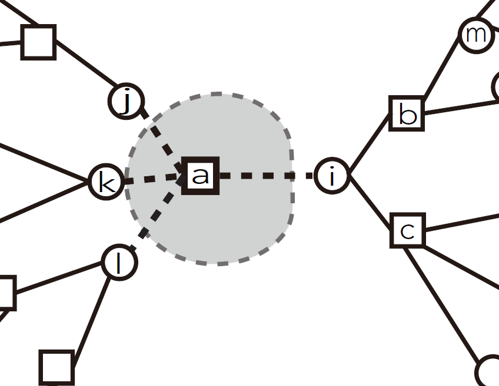
\includegraphics[width=\linewidth]{cavity_method_small_region.png}
\subcaption{}
\end{subfigure}
\begin{subfigure}{0.49\columnwidth}
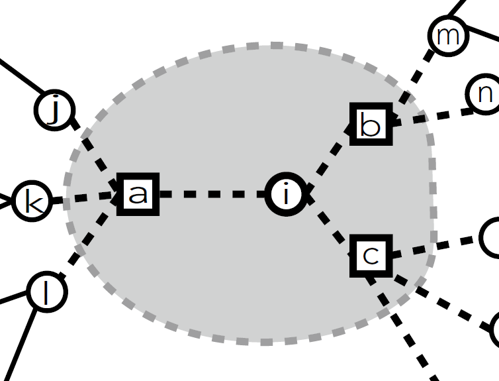
\includegraphics[width=\linewidth]{cavity_method_large_region.png}
\subcaption{}
\end{subfigure}
\caption{\label{fig:small_large_region} Figures showing cavities in regions of a factor graph. (a) shows a cavity in a small region while (b) shows one in a large region. Figures obtained from \cite{huang2021statistical_cavity}.}
\end{figure}
Small regions are single factor nodes while large regions are single variable nodes and its neighboring factor nodes.
% Notice that the most direct interactions between the variable nodes surrounding the cavities are severed. If the factor graph is sparse or the interactions are weak in the first place, then each surrounding variable node can be seen to be uncorrelated with another surrounding node. With this, the marginal distribution of all spin values can be decomposed into a product of the marginal distribution of every spin value for the surrounding variable nodes. 
A cavity allows one to talk about the magnetization of each surrounding variable node when the nodes in the cavity region doesn't exist and if the variable nodes are weakly correlated. If we then consider placing the nodes in the cavity region back, we can calculate the shift in free energy due to this change. By piecing up the shifts in free energy for all variable and factor nodes \cite{huang2021statistical_cavity_F} we can find an expression of the total free energy, $F$, of the system. 
\begin{align}
F&=\sum_i \Delta F_i + \sum_a \Delta F_a- \sum_a |\partial a| \Delta F_a
    \label{eq:cavity_F}\\
\Delta F_i &= -\frac{1}{\beta} \ln{\left( \sum_{\lambda = \pm} \prod_{b\in \partial i} \Lambda^{\lambda}_{b \rightarrow i} \right)}
    \label{eq:cavity_F_var_contri} \\
\Lambda^{\pm}_{b\rightarrow i}&=\cosh{(\beta J_b)}\left( 1 \pm \tanh{(\beta J_b)} \prod_{j\in \partial b \backslash i} m_{j\rightarrow b}   \right)
    \label{eq:Lambda_pm}\\
\Delta F_a &= -\frac{1}{\beta} \ln{\left[\cosh{(\beta J_a)}\left( 1+\tanh{(\beta J_a)} \prod_{i\in \partial a} m_{i\rightarrow a} \right) \right]}
    \label{eq:cavity_F_fac_contri}
\end{align}
where $m_{i\rightarrow a}$ is the magnetization of the $i$-th variable node when the $a$-th factor node is in a cavity, $\partial b \backslash i$ is the set of all variable nodes neighbouring the $b$-th factor node except the $i$-th variable node, $\Delta F_i$ and $\Delta F_a$ are respectively the shifts in free energy by adding the $i$-th variable node and the $a$-th factor node, and the last term in Equation \ref{eq:cavity_F} removes over-counting. 

It can be shown \cite{huang2021statistical_cavity_MP} that $m_{i\rightarrow a}$ can be calculated through Equation \ref{eq:mag_field} by iterating over Equations \ref{eq:h_MP} and \ref{eq:u_MP} until a fixed point is reached. At this fixed point, Equations \ref{eq:h_MP} and \ref{eq:u_MP} become a self-consistent equation, and interestingly the fixed point will also correspond to a stationary point of $F$. 
\begin{align}
m_{i\rightarrow a}&=\tanh{\beta h_{i\rightarrow a}}, \; \; \; \hat{m}_{a\rightarrow i}=\tanh{\beta u_{a\rightarrow i}} \label{eq:mag_field} \\
h_{i \rightarrow a}&=\frac{1}{\beta}\left( \sum_{b\in \partial i \backslash a} \beta u_{b \rightarrow i} \right) \label{eq:h_MP}\\
u_{a\rightarrow i}&=\frac{1}{\beta}\tanh^{-1}{\left[ \tanh{(\beta J_a)} \prod_{j \in \partial a \backslash i} \tanh{(\beta h_{j\rightarrow a}}) \right]} \label{eq:u_MP}
\end{align}
where $h_{i \rightarrow a}$ is the cavity local field, $u_{a\rightarrow i}$ is the cavity bias, and $\hat{m}_{a\rightarrow i}$ is the conjugate magnetization. Equations \ref{eq:h_MP} and \ref{eq:u_MP} are known as the message passing equations of the cavity fields. They are called message passing equations because they can be reduced to the message passing equations of belief propagation in Computer Science. Interestingly, they provide a very good physical picture for what is happening in a spin glass model. Equation \ref{eq:u_MP} is saying that the magnetization of the variable nodes neighbouring the factor node $a$ tells how the interaction encoded in the factor node should be. Equation \ref{eq:h_MP} is saying that the factor nodes neighbouring the variable node $i$ creates an effective local field at $i$, telling how the variable node should be magnetized. Hence, the variable nodes effectively communicate with each other recursively until an equilibrium is reached. This is exactly how a recurrent neural network should behave!

Finally, for every fixed point the free energy can be computed. With the fixed point that minimizes the free energy, the magnetization of each variable node can be calculated to solve the Ising problem:
$m_{i}=\tanh{\left( \sum_{b\in \partial i} \beta u_{b \rightarrow i} \right)}$.


\subsection{The Inverse Ising Problem and \\ Unsupervised Learning}
The inverse Ising problem \cite{huang2021statistical_inv_Ising} is formulated with a teacher-student scenario. $L$ samples of the teacher spin model's spin values is collected. Then, the student Ising model is tasked to reconstruct the weights of the teacher model from the samples, so as to reproduce spin values with the same statistics as the samples. It is clear that this fits closely the description of auto-associative self-supervised feature learning in Section \ref{sec:NN for ML}. 

In general, for continuous weights, the learning is done through gradient descent/ascent:
$    \delta J_{ij} \propto \langle s_i s_j \rangle_s - \langle s_i s_j \rangle_T $, 
where $\delta J_{ij}$ is a small nudge at each iteration step of gradient descent/ascent, $\langle \bullet \rangle_s$ is the sample average, and $\langle \bullet \rangle_T$ is the thermal average. To perform gradient descent/ascent, the Ising problem has to be solved at each iteration step. By extending the spin glass model to consider external fields ($H_i$), $\langle s_i s_j \rangle_T$ can be found through the fluctuation-dissipation theorem:
$\langle s_i s_j \rangle_T = \left[\frac{\partial m_j}{\partial H_i} + m_i m_j \right]_{\forall i, H_i=0} $.

\section{Simplest Model of Unsupervised Learning}

Having established the inverse Ising problem, it is a natural question to ask what are the factors affecting the efficacy of learning. Here we consider a simple model to investigate the roles played by the parameters $L$ and $\beta$. 

We introduce an RNN architecture known as the restricted Boltzmann machine (RBM). An RBM can be represented by a bipartite graph where there are only two layers in the neural network --- visible and hidden nodes. As the simplest model of unsupervised learning, we consider RBMs with only a single hidden node, $N$ visible nodes, and binary weights. This implies that there is a one-to-one correspondence between the visible nodes and the weights. Thus, the Hamiltonian of our simple model can be written as: 
\begin{align}
    \mathcal{H}\left((s_i)_{i=1}^{N},s_0 \right) = -\sum_{i=1}^{N} s_i J_{i} s_0, \; \; s_i,s_0,J_i \in \{1,-1\} \label{eq:RBM_H}
\end{align}
where $s_0$ is the spin value of the hidden node. \textit{Independent} samples produced from the teacher RBM would only contain the spin values of the visible nodes and the student RBM is tasked to reconstruct the weights of the teacher RBM at the same temperature. Since this RBM has discrete binary weights, gradient descent/ascent no longer makes sense. Instead, a Bayesian learning framework can be adopted --- the set of predicted weights, $\{\hat{J_i}\}$ should maximize the posterior probability:
\begin{align}
\Pr{\left(J_i \middle| \left\{(s_i)_{i=1}^{N}\right\}_{a=1}^L \right)}=\frac{1}{Z}\prod_{a=1}^L \cosh{\left( \frac{\beta}{\sqrt{N}} \sum_{i=1}^{N} J_i s_{i,a} \right)}
\label{eq:posterior_prob}
\end{align}
which can be derived by marginalizing the joint conditional probability $\Pr{\left( \left\{(s_i)_{i=0}^{N}\right\}_{a=1}^L  \middle|  J_i \right) }$ obtained from Equation \ref{eq:RBM_H} through the canonical ensemble and applying Bayes' theorem \cite{huang2021statistical_boltzmannM,huang2021statistical_simplestModel}. Then, notice that Equation \ref{eq:posterior_prob} can be easily cast into a factor graph representation, with $L$ factor nodes indexed by $a$ and $N$ variable nodes indexed by $i$ (Caution: the weights are now the variable nodes instead!). With appropriate approximations in the thermodynamic limit, the cavity method described by Equations \ref{eq:mag_field} - \ref{eq:u_MP} can be implemented with little modifications \cite{huang2016unsupervised,huang2021statistical_boltzmannM}. 

Finally, the weights can be reconstructed through 
$\hat{J_i} = \arg \max_{J_i} \left(\frac{1+m_i J_i}{2}\right) = \sgn{(m_i)}$,
where $m_i$ is the magnetization of the $i$-th variable node.

\subsection{Temperature, Data Density, and Phase Transition}

The efficacy of learning can be analyzed through the overlaps $q=\left\langle \left| \overline{  J_i^{\text{true}} \hat{J_i}  } \right| \right\rangle_{d,s}$ and $Q=  \overline{{m_i}^2}  $, where $\left\langle \bullet  \right\rangle_{d,s}$ is a disorder average over a random set of realizations while $\overline{\bullet}$ is the average over all variable nodes. $q$ measures how well the student RBM's predicted weights overlap with the teacher RBM. A $q$ near zero indicates that the student RBM is performing not much better than random guessing. The modulus appearing in the expression for $q$ emphasizes that having a very low accuracy in predicting the weights is in fact favourable. A student RBM with a perfectly wrong feature matrix will yield exactly the same output spin value statistics as a perfectly correct student RBM. This is the result of $Z_2$ symmetry present in the model with no external fields. On the other hand, $Q$ is closely related to the Edwards-Anderson order parameter, $\hat{q}_{\rho \sigma}$, from the replica method. 

Figure \ref{fig:phase} depicts how $q$ increases with the data density $\alpha=L/N$ after a critical $\alpha_c$ governed by temperature. Better performance with increasing $\alpha$ is expected as learning is always more effective with more data. Interesting questions are then what effects $\beta$ has and why $Q$ exhibits the same behaviour. We only attempt to answer the former here. Figure \ref{fig:metropolis} shows how the Gibbs sampling of the teacher RBM is done with the Metropolis algorithm. At higher temperature, the equilibrium Hamiltonian has large fluctuations, so the sample generated carry more random noise. This offers intuitive explanation of why high temperature negatively affects $q$.
\begin{figure}[]
\begin{subfigure}{0.49\columnwidth}
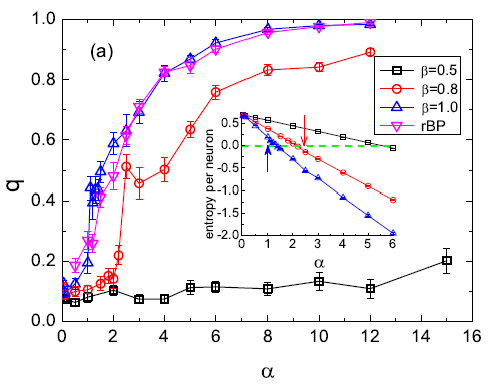
\includegraphics[width=\linewidth]{q against alpha.png}
\subcaption{}
\end{subfigure}
\begin{subfigure}{0.49\columnwidth}
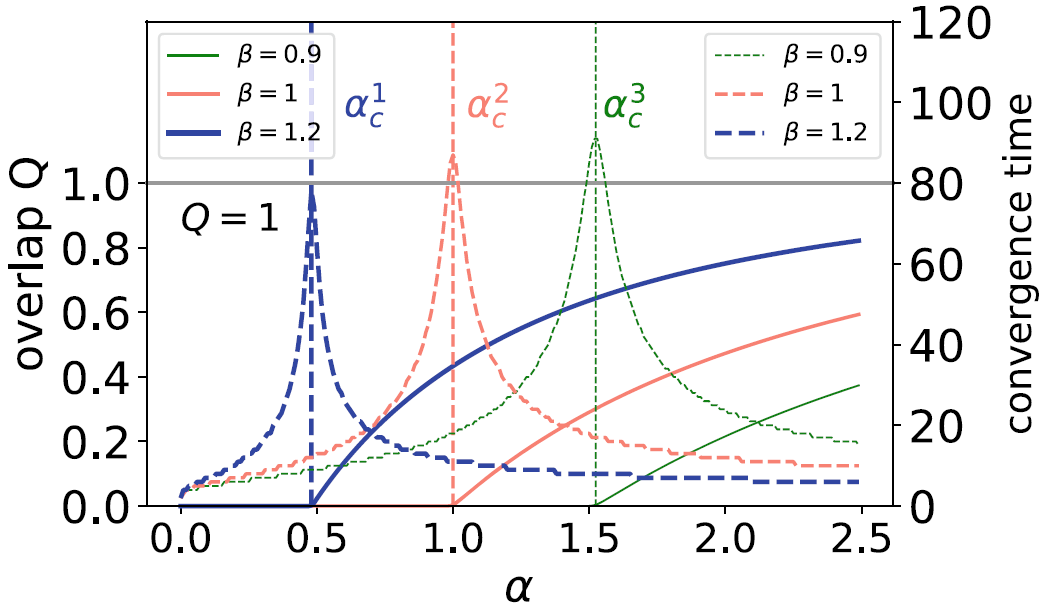
\includegraphics[width=\linewidth]{big Q against alpha.png}
\subcaption{}
\end{subfigure}
\caption{\label{fig:phase} Phase transition in learning. (a) is a plot of $q$ against $\alpha$ at different $\beta$ for the blue, orange and black lines. Plot from \cite{huang2016unsupervised}. The inset depicts entropy per neuron which we do not discuss here. (b) shows a plot of $Q$ against the same with different $\beta$ for the solid lines from \cite{huang2021statistical_simplestModel}. Dashed lines show convergence time of message passing which we do not discuss here.}
\end{figure}
\begin{figure}[]
\begin{subfigure}{0.49\columnwidth}
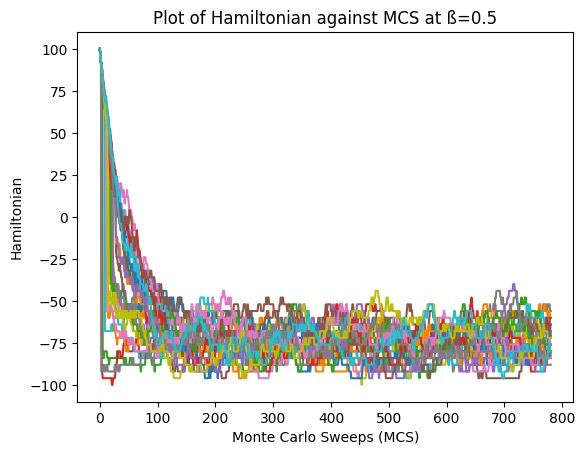
\includegraphics[width=\linewidth]{metropolis_beta0.5.jpeg}
\subcaption{}
\end{subfigure}
\begin{subfigure}{0.49\columnwidth}
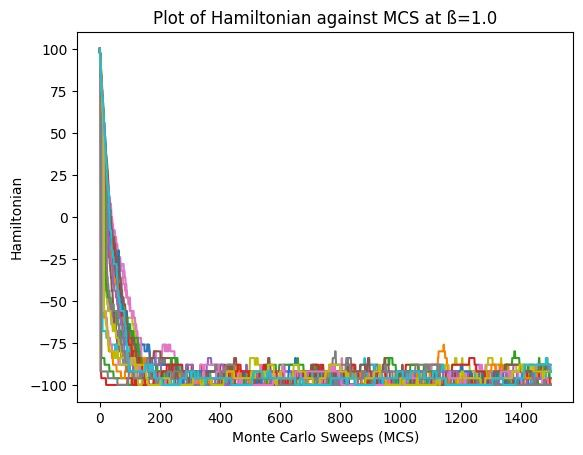
\includegraphics[width=\linewidth]{metropolis_beta1.jpeg}
\subcaption{}
\end{subfigure}
\caption{\label{fig:metropolis} Hamiltonian values of an ensemble of random walks against Monte Carlo sweeps in Metropolis algorithm used for Gibbs sampling of teacher RBM. (a) is at $\beta=0.5$ and (b) is at $\beta=1$.}
\end{figure}


\section{Conclusions and Points of Further Interest}

In this paper, we have demonstrated that spin glass models are RNNs and the inverse Ising problem is a form of unsupervised learning. We also discussed how $\alpha$ and $\beta$ affects the effectiveness of learning. 

However, we did not discuss the connection between $Q$ and $q$, which lies in the physics of replica symmetry breaking \cite{huang2021statistical_replica_sym_break,Castellani_2005}. Replica symmetry breaking together with Goldstone's theorem also yield other interesting concepts \cite{Fedorenko_2003}. With regards to phase transitions, the reader may also be interested in the analysis of neural networks with other tools like renormalization groups \cite{li2018neural}. 

Lastly, we note that the model we have treated here is way too simple compared to modern neural networks used for, as an example, deep learning.  Understanding the inner-workings of complex neural networks is ongoing work. Some recent work are available in that regard \cite{doi:10.1146/annurev-conmatphys-031119-050745}.


\newpage
% \section{Simulation}
% With the mathematical framework established, we can start to run simulations to obtain samples from the truth feature vector of a random teacher model. For the student model to learn from samples, we will employ cavity method to reconstruct the feature vector of the teacher model. Comparing with the truth feature vector with the reconstructed feature vector, we will examine the accuracy of the result and investigate its dependence on "temperature".
% \subsection{Monte Carlo Simulation and Metropolis Algorithm}
% To generate the \textit{independent} samples from the teacher RBM, we would need to create a teacher RBM. The RBM is a simple bipartite graph with a single hidden node and N visible (variable) nodes, hence we can construct a simple adjacency matrix to represent the graph. To do so, we generate a random feature vector, and using the characteristic of a bipartite graph, the adjacency matrix can be easily constructed as there is only one hidden node.\\
% To simulate the trajectory of the teacher node traversing to equilibrium, we would need to allow it to undergo random walks through the Monte Carlo method. The Monte Carlo method employs the concept of the law of large numbers to obtain the expectation of a random variable\cite{spall2003estimation}. For this project, a Monte Carlo method in statistical physics is called Metropolis Algorithm. The Metropolis algorithm is used when obtaining the probability distribution is non-trivial\cite{rosenbluth2003genesis}.

% \begin{itemize}
%     \item Scan Size
%     \item Scan Rate
%     \item Pixel Size
%     \item Force Point (Contact Mode only)
%     \item Set Point (Non-Contact Mode only)
% \end{itemize}

% \subsection{Message Passing for Inverse Ising Problem}



% \section{Conclusion}


% \subsection{\label{sec:level2}Second-level heading: Formatting}

% This file may be formatted in either the \texttt{preprint} or
% \texttt{reprint} style. \texttt{reprint} format mimics final journal output. 
% Either format may be used for submission purposes. \texttt{letter} sized paper should
% be used when submitting to APS journals.

% \subsubsection{Wide text (A level-3 head)}
% The \texttt{widetext} environment will make the text the width of the
% full page, as on page~\pageref{eq:wideeq}. (Note the use the
% \verb+\pageref{#1}+ command to refer to the page number.) 
% \paragraph{Note (Fourth-level head is run in)}
% The width-changing commands only take effect in two-column formatting. 
% There is no effect if text is in a single column.

% \subsection{\label{sec:citeref}Citations and References}
% A citation in text uses the command \verb+\cite{#1}+ or
% \verb+\onlinecite{#1}+ and refers to an entry in the bibliography. 
% An entry in the bibliography is a reference to another document.

% \subsubsection{Citations}
% Because REV\TeX\ uses the \verb+natbib+ package of Patrick Daly, 
% the entire repertoire of commands in that package are available for your document;
% see the \verb+natbib+ documentation for further details. Please note that
% REV\TeX\ requires version 8.31a or later of \verb+natbib+.

% \paragraph{Syntax}
% The argument of \verb+\cite+ may be a single \emph{key}, 
% or may consist of a comma-separated list of keys.
% The citation \emph{key} may contain 
% letters, numbers, the dash (-) character, or the period (.) character. 
% New with natbib 8.3 is an extension to the syntax that allows for 
% a star (*) form and two optional arguments on the citation key itself.
% The syntax of the \verb+\cite+ command is thus (informally stated)
% \begin{quotation}\flushleft\leftskip1em
% \verb+\cite+ \verb+{+ \emph{key} \verb+}+, or\\
% \verb+\cite+ \verb+{+ \emph{optarg+key} \verb+}+, or\\
% \verb+\cite+ \verb+{+ \emph{optarg+key} \verb+,+ \emph{optarg+key}\ldots \verb+}+,
% \end{quotation}\noindent
% where \emph{optarg+key} signifies 
% \begin{quotation}\flushleft\leftskip1em
% \emph{key}, or\\
% \texttt{*}\emph{key}, or\\
% \texttt{[}\emph{pre}\texttt{]}\emph{key}, or\\
% \texttt{[}\emph{pre}\texttt{]}\texttt{[}\emph{post}\texttt{]}\emph{key}, or even\\
% \texttt{*}\texttt{[}\emph{pre}\texttt{]}\texttt{[}\emph{post}\texttt{]}\emph{key}.
% \end{quotation}\noindent
% where \emph{pre} and \emph{post} is whatever text you wish to place 
% at the beginning and end, respectively, of the bibliographic reference
% (see Ref.~[\onlinecite{witten2001}] and the two under Ref.~[\onlinecite{feyn54}]).
% (Keep in mind that no automatic space or punctuation is applied.)
% It is highly recommended that you put the entire \emph{pre} or \emph{post} portion 
% within its own set of braces, for example: 
% \verb+\cite+ \verb+{+ \texttt{[} \verb+{+\emph{text}\verb+}+\texttt{]}\emph{key}\verb+}+.
% The extra set of braces will keep \LaTeX\ out of trouble if your \emph{text} contains the comma (,) character.

% The star (*) modifier to the \emph{key} signifies that the reference is to be 
% merged with the previous reference into a single bibliographic entry, 
% a common idiom in APS and AIP articles (see below, Ref.~[\onlinecite{epr}]). 
% When references are merged in this way, they are separated by a semicolon instead of 
% the period (full stop) that would otherwise appear.

% \paragraph{Eliding repeated information}
% When a reference is merged, some of its fields may be elided: for example, 
% when the author matches that of the previous reference, it is omitted. 
% If both author and journal match, both are omitted.
% If the journal matches, but the author does not, the journal is replaced by \emph{ibid.},
% as exemplified by Ref.~[\onlinecite{epr}]. 
% These rules embody common editorial practice in APS and AIP journals and will only
% be in effect if the markup features of the APS and AIP Bib\TeX\ styles is employed.

% \paragraph{The options of the cite command itself}
% Please note that optional arguments to the \emph{key} change the reference in the bibliography, 
% not the citation in the body of the document. 
% For the latter, use the optional arguments of the \verb+\cite+ command itself:
% \verb+\cite+ \texttt{*}\allowbreak
% \texttt{[}\emph{pre-cite}\texttt{]}\allowbreak
% \texttt{[}\emph{post-cite}\texttt{]}\allowbreak
% \verb+{+\emph{key-list}\verb+}+.

% \subsubsection{Example citations}
% By default, citations are numerical\cite{Beutler1994}.
% Author-year citations are used when the journal is RMP. 
% To give a textual citation, use \verb+\onlinecite{#1}+: 
% Refs.~\onlinecite{[][{, and references therein}]witten2001,Bire82}. 
% By default, the \texttt{natbib} package automatically sorts your citations into numerical order and ``compresses'' runs of three or more consecutive numerical citations.
% REV\TeX\ provides the ability to automatically change the punctuation when switching between journal styles that provide citations in square brackets and those that use a superscript style instead. This is done through the \texttt{citeautoscript} option. For instance, the journal style \texttt{prb} automatically invokes this option because \textit{Physical 
% Review B} uses superscript-style citations. The effect is to move the punctuation, which normally comes after a citation in square brackets, to its proper position before the superscript. 
% To illustrate, we cite several together 
% \cite{[See the explanation of time travel in ]feyn54,*[The classical relativistic treatment of ][ is a relative classic]epr,witten2001,Berman1983,Davies1998,Bire82}, 
% and once again in different order (Refs.~\cite{epr,feyn54,Bire82,Berman1983,witten2001,Davies1998}). 
% Note that the citations were both compressed and sorted. Futhermore, running this sample file under the \texttt{prb} option will move the punctuation to the correct place.

% When the \verb+prb+ class option is used, the \verb+\cite{#1}+ command
% displays the reference's number as a superscript rather than in
% square brackets. Note that the location of the \verb+\cite{#1}+
% command should be adjusted for the reference style: the superscript
% references in \verb+prb+ style must appear after punctuation;
% otherwise the reference must appear before any punctuation. This
% sample was written for the regular (non-\texttt{prb}) citation style.
% The command \verb+\onlinecite{#1}+ in the \texttt{prb} style also
% displays the reference on the baseline.

% \subsubsection{References}
% A reference in the bibliography is specified by a \verb+\bibitem{#1}+ command
% with the same argument as the \verb+\cite{#1}+ command.
% \verb+\bibitem{#1}+ commands may be crafted by hand or, preferably,
% generated by Bib\TeX. 
% REV\TeX~4.2 includes Bib\TeX\ style files
% \verb+apsrev4-2.bst+, \verb+apsrmp4-2.bst+ appropriate for
% \textit{Physical Review} and \textit{Reviews of Modern Physics},
% respectively.

% \subsubsection{Example references}
% This sample file employs the \verb+\bibliography+ command, 
% which formats the \texttt{\jobname .bbl} file
% and specifies which bibliographic databases are to be used by Bib\TeX\ 
% (one of these should be by arXiv convention \texttt{\jobname .bib}).
% Running Bib\TeX\ (via \texttt{bibtex \jobname}) 
% after the first pass of \LaTeX\ produces the file
% \texttt{\jobname .bbl} which contains the automatically formatted
% \verb+\bibitem+ commands (including extra markup information via
% \verb+\bibinfo+ and \verb+\bibfield+ commands). 
% If not using Bib\TeX, you will have to create the \verb+thebibiliography+ environment 
% and its \verb+\bibitem+ commands by hand.

% Numerous examples of the use of the APS bibliographic entry types appear in the bibliography of this sample document.
% You can refer to the \texttt{\jobname .bib} file, 
% and compare its information to the formatted bibliography itself.


% \section{Math and Equations}
% Inline math may be typeset using the \verb+$+ delimiters. Bold math
% symbols may be achieved using the \verb+bm+ package and the
% \verb+\bm{#1}+ command it supplies. For instance, a bold $\alpha$ can
% be typeset as \verb+$\bm{\alpha}$+ giving $\bm{\alpha}$. Fraktur and
% Blackboard (or open face or double struck) characters should be
% typeset using the \verb+\mathfrak{#1}+ and \verb+\mathbb{#1}+ commands
% respectively. Both are supplied by the \texttt{amssymb} package. For
% example, \verb+$\mathbb{R}$+ gives $\mathbb{R}$ and
% \verb+$\mathfrak{G}$+ gives $\mathfrak{G}$

% In \LaTeX\ there are many different ways to display equations, and a
% few preferred ways are noted below. Displayed math will center by
% default. Use the class option \verb+fleqn+ to flush equations left.

% Below we have numbered single-line equations; this is the most common
% type of equation in \textit{Physical Review}:
% \begin{eqnarray}
% \chi_+(p)\alt{\bf [}2|{\bf p}|(|{\bf p}|+p_z){\bf ]}^{-1/2}
% \left(
% \begin{array}{c}
% |{\bf p}|+p_z\\
% px+ip_y
% \end{array}\right)\;,
% \\
% \left\{%
%  \openone234567890abc123\alpha\beta\gamma\delta1234556\alpha\beta
%  \frac{1\sum^{a}_{b}}{A^2}%
% \right\}%
% \label{eq:one}.
% \end{eqnarray}
% Note the open one in Eq.~(\ref{eq:one}).

% Not all numbered equations will fit within a narrow column this
% way. The equation number will move down automatically if it cannot fit
% on the same line with a one-line equation:
% \begin{equation}
% \left\{
%  ab12345678abc123456abcdef\alpha\beta\gamma\delta1234556\alpha\beta
%  \frac{1\sum^{a}_{b}}{A^2}%
% \right\}.
% \end{equation}

% When the \verb+\label{#1}+ command is used [cf. input for
% Eq.~(\ref{eq:one})], the equation can be referred to in text without
% knowing the equation number that \TeX\ will assign to it. Just
% use \verb+\ref{#1}+, where \verb+#1+ is the same name that used in
% the \verb+\label{#1}+ command.

% Unnumbered single-line equations can be typeset
% using the \verb+\[+, \verb+\]+ format:
% \[g^+g^+ \rightarrow g^+g^+g^+g^+ \dots ~,~~q^+q^+\rightarrow
% q^+g^+g^+ \dots ~. \]


% \subsection{Multiline equations}

% Multiline equations are obtained by using the \verb+eqnarray+
% environment.  Use the \verb+\nonumber+ command at the end of each line
% to avoid assigning a number:
% \begin{eqnarray}
% {\cal M}=&&ig_Z^2(4E_1E_2)^{1/2}(l_i^2)^{-1}
% \delta_{\sigma_1,-\sigma_2}
% (g_{\sigma_2}^e)^2\chi_{-\sigma_2}(p_2)\nonumber\\
% &&\times
% [\epsilon_jl_i\epsilon_i]_{\sigma_1}\chi_{\sigma_1}(p_1),
% \end{eqnarray}
% \begin{eqnarray}
% \sum \vert M^{\text{viol}}_g \vert ^2&=&g^{2n-4}_S(Q^2)~N^{n-2}
%         (N^2-1)\nonumber \\
%  & &\times \left( \sum_{i<j}\right)
%   \sum_{\text{perm}}
%  \frac{1}{S_{12}}
%  \frac{1}{S_{12}}
%  \sum_\tau c^f_\tau~.
% \end{eqnarray}
% \textbf{Note:} Do not use \verb+\label{#1}+ on a line of a multiline
% equation if \verb+\nonumber+ is also used on that line. Incorrect
% cross-referencing will result. Notice the use \verb+\text{#1}+ for
% using a Roman font within a math environment.

% To set a multiline equation without \emph{any} equation
% numbers, use the \verb+\begin{eqnarray*}+,
% \verb+\end{eqnarray*}+ format:
% \begin{eqnarray*}
% \sum \vert M^{\text{viol}}_g \vert ^2&=&g^{2n-4}_S(Q^2)~N^{n-2}
%         (N^2-1)\\
%  & &\times \left( \sum_{i<j}\right)
%  \left(
%   \sum_{\text{perm}}\frac{1}{S_{12}S_{23}S_{n1}}
%  \right)
%  \frac{1}{S_{12}}~.
% \end{eqnarray*}

% To obtain numbers not normally produced by the automatic numbering,
% use the \verb+\tag{#1}+ command, where \verb+#1+ is the desired
% equation number. For example, to get an equation number of
% (\ref{eq:mynum}),
% \begin{equation}
% g^+g^+ \rightarrow g^+g^+g^+g^+ \dots ~,~~q^+q^+\rightarrow
% q^+g^+g^+ \dots ~. \tag{2.6$'$}\label{eq:mynum}
% \end{equation}

% \paragraph{A few notes on \texttt{tag}s} 
% \verb+\tag{#1}+ requires the \texttt{amsmath} package. 
% Place the \verb+\tag{#1}+ command before the \verb+\label{#1}+, if any. 
% The numbering produced by \verb+\tag{#1}+ \textit{does not affect} 
% the automatic numbering in REV\TeX; 
% therefore, the number must be known ahead of time, 
% and it must be manually adjusted if other equations are added. 
% \verb+\tag{#1}+ works with both single-line and multiline equations. 
% \verb+\tag{#1}+ should only be used in exceptional cases---%
% do not use it to number many equations in your paper. 
% Please note that this feature of the \texttt{amsmath} package
% is \emph{not} compatible with the \texttt{hyperref} (6.77u) package.

% Enclosing display math within
% \verb+\begin{subequations}+ and \verb+\end{subequations}+ will produce
% a set of equations that are labeled with letters, as shown in
% Eqs.~(\ref{subeq:1}) and (\ref{subeq:2}) below.
% You may include any number of single-line and multiline equations,
% although it is probably not a good idea to follow one display math
% directly after another.
% \begin{subequations}
% \label{eq:whole}
% \begin{eqnarray}
% {\cal M}=&&ig_Z^2(4E_1E_2)^{1/2}(l_i^2)^{-1}
% (g_{\sigma_2}^e)^2\chi_{-\sigma_2}(p_2)\nonumber\\
% &&\times
% [\epsilon_i]_{\sigma_1}\chi_{\sigma_1}(p_1).\label{subeq:2}
% \end{eqnarray}
% \begin{equation}
% \left\{
%  abc123456abcdef\alpha\beta\gamma\delta1234556\alpha\beta
%  \frac{1\sum^{a}_{b}}{A^2}
% \right\},\label{subeq:1}
% \end{equation}
% \end{subequations}
% Giving a \verb+\label{#1}+ command directly after the \verb+\begin{subequations}+, 
% allows you to reference all the equations in the \texttt{subequations} environment. 
% For example, the equations in the preceding subequations environment were
% Eqs.~(\ref{eq:whole}).

% \subsubsection{Wide equations}
% The equation that follows is set in a wide format, i.e., it spans the full page. 
% The wide format is reserved for long equations
% that cannot easily be set in a single column:
% \begin{widetext}
% \begin{equation}
% {\cal R}^{(\text{d})}=
%  g_{\sigma_2}^e
%  \left(
%    \frac{[\Gamma^Z(3,21)]_{\sigma_1}}{Q_{12}^2-M_W^2}
%   +\frac{[\Gamma^Z(13,2)]_{\sigma_1}}{Q_{13}^2-M_W^2}
%  \right)
%  + x_WQ_e
%  \left(
%    \frac{[\Gamma^\gamma(3,21)]_{\sigma_1}}{Q_{12}^2-M_W^2}
%   +\frac{[\Gamma^\gamma(13,2)]_{\sigma_1}}{Q_{13}^2-M_W^2}
%  \right)\;. 
%  \label{eq:wideeq}
% \end{equation}
% \end{widetext}
% This is typed to show how the output appears in wide format.
% (Incidentally, since there is no blank line between the \texttt{equation} environment above 
% and the start of this paragraph, this paragraph is not indented.)

% \section{Cross-referencing}
% REV\TeX{} will automatically number such things as
% sections, footnotes, equations, figure captions, and table captions. 
% In order to reference them in text, use the
% \verb+\label{#1}+ and \verb+\ref{#1}+ commands. 
% To reference a particular page, use the \verb+\pageref{#1}+ command.

% The \verb+\label{#1}+ should appear 
% within the section heading, 
% within the footnote text, 
% within the equation, or 
% within the table or figure caption. 
% The \verb+\ref{#1}+ command
% is used in text at the point where the reference is to be displayed.  
% Some examples: Section~\ref{sec:level1} on page~\pageref{sec:level1},
% Table~\ref{tab:table1},%
% \begin{table}[b]%The best place to locate the table environment is directly after its first reference in text
% \caption{\label{tab:table1}%
% A table that fits into a single column of a two-column layout. 
% Note that REV\TeX~4 adjusts the intercolumn spacing so that the table fills the
% entire width of the column. Table captions are numbered
% automatically. 
% This table illustrates left-, center-, decimal- and right-aligned columns,
% along with the use of the \texttt{ruledtabular} environment which sets the 
% Scotch (double) rules above and below the alignment, per APS style.
% }
% \begin{ruledtabular}
% \begin{tabular}{lcdr}
% \textrm{Left\footnote{Note a.}}&
% \textrm{Centered\footnote{Note b.}}&
% \multicolumn{1}{c}{\textrm{Decimal}}&
% \textrm{Right}\\
% \colrule
% 1 & 2 & 3.001 & 4\\
% 10 & 20 & 30 & 40\\
% 100 & 200 & 300.0 & 400\\
% \end{tabular}
% \end{ruledtabular}
% \end{table}
% and Fig.~\ref{fig:epsart}.%
% \begin{figure}[b]
% \includegraphics{fig_1}% Here is how to import EPS art
% \caption{\label{fig:epsart} A figure caption. The figure captions are
% automatically numbered.}
% \end{figure}

% \section{Floats: Figures, Tables, Videos, etc.}
% Figures and tables are usually allowed to ``float'', which means that their
% placement is determined by \LaTeX, while the document is being typeset. 

% Use the \texttt{figure} environment for a figure, the \texttt{table} environment for a table.
% In each case, use the \verb+\caption+ command within to give the text of the
% figure or table caption along with the \verb+\label+ command to provide
% a key for referring to this figure or table.
% The typical content of a figure is an image of some kind; 
% that of a table is an alignment.%
% \begin{figure*}
% \includegraphics{fig_2}% Here is how to import EPS art
% \caption{\label{fig:wide}Use the figure* environment to get a wide
% figure that spans the page in \texttt{twocolumn} formatting.}
% \end{figure*}
% \begin{table*}
% \caption{\label{tab:table3}This is a wide table that spans the full page
% width in a two-column layout. It is formatted using the
% \texttt{table*} environment. It also demonstates the use of
% \textbackslash\texttt{multicolumn} in rows with entries that span
% more than one column.}
% \begin{ruledtabular}
% \begin{tabular}{ccccc}
%  &\multicolumn{2}{c}{$D_{4h}^1$}&\multicolumn{2}{c}{$D_{4h}^5$}\\
%  Ion&1st alternative&2nd alternative&lst alternative
% &2nd alternative\\ \hline
%  K&$(2e)+(2f)$&$(4i)$ &$(2c)+(2d)$&$(4f)$ \\
%  Mn&$(2g)$\footnote{The $z$ parameter of these positions is $z\sim\frac{1}{4}$.}
%  &$(a)+(b)+(c)+(d)$&$(4e)$&$(2a)+(2b)$\\
%  Cl&$(a)+(b)+(c)+(d)$&$(2g)$\footnotemark[1]
%  &$(4e)^{\text{a}}$\\
%  He&$(8r)^{\text{a}}$&$(4j)^{\text{a}}$&$(4g)^{\text{a}}$\\
%  Ag& &$(4k)^{\text{a}}$& &$(4h)^{\text{a}}$\\
% \end{tabular}
% \end{ruledtabular}
% \end{table*}

% Insert an image using either the \texttt{graphics} or
% \texttt{graphix} packages, which define the \verb+\includegraphics{#1}+ command.
% (The two packages differ in respect of the optional arguments 
% used to specify the orientation, scaling, and translation of the image.) 
% To create an alignment, use the \texttt{tabular} environment. 

% The best place to locate the \texttt{figure} or \texttt{table} environment
% is immediately following its first reference in text; this sample document
% illustrates this practice for Fig.~\ref{fig:epsart}, which
% shows a figure that is small enough to fit in a single column. 

% In exceptional cases, you will need to move the float earlier in the document, as was done
% with Table~\ref{tab:table3}: \LaTeX's float placement algorithms need to know
% about a full-page-width float earlier. 

% Fig.~\ref{fig:wide}
% has content that is too wide for a single column,
% so the \texttt{figure*} environment has been used.%
% \begin{table}[b]
% \caption{\label{tab:table4}%
% Numbers in columns Three--Five are aligned with the ``d'' column specifier 
% (requires the \texttt{dcolumn} package). 
% Non-numeric entries (those entries without a ``.'') in a ``d'' column are aligned on the decimal point. 
% Use the ``D'' specifier for more complex layouts. }
% \begin{ruledtabular}
% \begin{tabular}{ccddd}
% One&Two&
% \multicolumn{1}{c}{\textrm{Three}}&
% \multicolumn{1}{c}{\textrm{Four}}&
% \multicolumn{1}{c}{\textrm{Five}}\\
% %\mbox{Three}&\mbox{Four}&\mbox{Five}\\
% \hline
% one&two&\mbox{three}&\mbox{four}&\mbox{five}\\
% He&2& 2.77234 & 45672. & 0.69 \\
% C\footnote{Some tables require footnotes.}
%   &C\footnote{Some tables need more than one footnote.}
%   & 12537.64 & 37.66345 & 86.37 \\
% \end{tabular}
% \end{ruledtabular}
% \end{table}

% The content of a table is typically a \texttt{tabular} environment, 
% giving rows of type in aligned columns. 
% Column entries separated by \verb+&+'s, and 
% each row ends with \textbackslash\textbackslash. 
% The required argument for the \texttt{tabular} environment
% specifies how data are aligned in the columns. 
% For instance, entries may be centered, left-justified, right-justified, aligned on a decimal
% point. 
% Extra column-spacing may be be specified as well, 
% although REV\TeX~4 sets this spacing so that the columns fill the width of the
% table. Horizontal rules are typeset using the \verb+\hline+
% command. The doubled (or Scotch) rules that appear at the top and
% bottom of a table can be achieved enclosing the \texttt{tabular}
% environment within a \texttt{ruledtabular} environment. Rows whose
% columns span multiple columns can be typeset using the
% \verb+\multicolumn{#1}{#2}{#3}+ command (for example, see the first
% row of Table~\ref{tab:table3}).%

% Tables~\ref{tab:table1}, \ref{tab:table3}, \ref{tab:table4}, and \ref{tab:table2}%
% \begin{table}[b]
% \caption{\label{tab:table2}
% A table with numerous columns that still fits into a single column. 
% Here, several entries share the same footnote. 
% Inspect the \LaTeX\ input for this table to see exactly how it is done.}
% \begin{ruledtabular}
% \begin{tabular}{cccccccc}
%  &$r_c$ (\AA)&$r_0$ (\AA)&$\kappa r_0$&
%  &$r_c$ (\AA) &$r_0$ (\AA)&$\kappa r_0$\\
% \hline
% Cu& 0.800 & 14.10 & 2.550 &Sn\footnotemark[1]
% & 0.680 & 1.870 & 3.700 \\
% Ag& 0.990 & 15.90 & 2.710 &Pb\footnotemark[2]
% & 0.450 & 1.930 & 3.760 \\
% Au& 1.150 & 15.90 & 2.710 &Ca\footnotemark[3]
% & 0.750 & 2.170 & 3.560 \\
% Mg& 0.490 & 17.60 & 3.200 &Sr\footnotemark[4]
% & 0.900 & 2.370 & 3.720 \\
% Zn& 0.300 & 15.20 & 2.970 &Li\footnotemark[2]
% & 0.380 & 1.730 & 2.830 \\
% Cd& 0.530 & 17.10 & 3.160 &Na\footnotemark[5]
% & 0.760 & 2.110 & 3.120 \\
% Hg& 0.550 & 17.80 & 3.220 &K\footnotemark[5]
% &  1.120 & 2.620 & 3.480 \\
% Al& 0.230 & 15.80 & 3.240 &Rb\footnotemark[3]
% & 1.330 & 2.800 & 3.590 \\
% Ga& 0.310 & 16.70 & 3.330 &Cs\footnotemark[4]
% & 1.420 & 3.030 & 3.740 \\
% In& 0.460 & 18.40 & 3.500 &Ba\footnotemark[5]
% & 0.960 & 2.460 & 3.780 \\
% Tl& 0.480 & 18.90 & 3.550 & & & & \\
% \end{tabular}
% \end{ruledtabular}
% \footnotetext[1]{Here's the first, from Ref.~\onlinecite{feyn54}.}
% \footnotetext[2]{Here's the second.}
% \footnotetext[3]{Here's the third.}
% \footnotetext[4]{Here's the fourth.}
% \footnotetext[5]{And etc.}
% \end{table}
% show various effects.
% A table that fits in a single column employs the \texttt{table}
% environment. 
% Table~\ref{tab:table3} is a wide table, set with the \texttt{table*} environment. 
% Long tables may need to break across pages. 
% The most straightforward way to accomplish this is to specify
% the \verb+[H]+ float placement on the \texttt{table} or
% \texttt{table*} environment. 
% However, the \LaTeXe\ package \texttt{longtable} allows headers and footers to be specified for each page of the table. 
% A simple example of the use of \texttt{longtable} can be found
% in the file \texttt{summary.tex} that is included with the REV\TeX~4
% distribution.

% There are two methods for setting footnotes within a table (these
% footnotes will be displayed directly below the table rather than at
% the bottom of the page or in the bibliography). The easiest
% and preferred method is just to use the \verb+\footnote{#1}+
% command. This will automatically enumerate the footnotes with
% lowercase roman letters. However, it is sometimes necessary to have
% multiple entries in the table share the same footnote. In this case,
% there is no choice but to manually create the footnotes using
% \verb+\footnotemark[#1]+ and \verb+\footnotetext[#1]{#2}+.
% \texttt{\#1} is a numeric value. Each time the same value for
% \texttt{\#1} is used, the same mark is produced in the table. The
% \verb+\footnotetext[#1]{#2}+ commands are placed after the \texttt{tabular}
% environment. Examine the \LaTeX\ source and output for
% Tables~\ref{tab:table1} and \ref{tab:table2}
% for examples.

% Video~\ref{vid:PRSTPER.4.010101} 
% illustrates several features new with REV\TeX4.2,
% starting with the \texttt{video} environment, which is in the same category with
% \texttt{figure} and \texttt{table}.%
% \begin{video}
% \href{http://prst-per.aps.org/multimedia/PRSTPER/v4/i1/e010101/e010101_vid1a.mpg}{\includegraphics{vid_1a}}%
%  \quad
% \href{http://prst-per.aps.org/multimedia/PRSTPER/v4/i1/e010101/e010101_vid1b.mpg}{\includegraphics{vid_1b}}
%  \setfloatlink{http://link.aps.org/multimedia/PRSTPER/v4/i1/e010101}%
%  \caption{\label{vid:PRSTPER.4.010101}%
%   Students explain their initial idea about Newton's third law to a teaching assistant. 
%   Clip (a): same force.
%   Clip (b): move backwards.
%  }%
% \end{video}
% The \verb+\setfloatlink+ command causes the title of the video to be a hyperlink to the
% indicated URL; it may be used with any environment that takes the \verb+\caption+
% command.
% The \verb+\href+ command has the same significance as it does in the context of
% the \texttt{hyperref} package: the second argument is a piece of text to be 
% typeset in your document; the first is its hyperlink, a URL.

% \textit{Physical Review} style requires that the initial citation of
% figures or tables be in numerical order in text, so don't cite
% Fig.~\ref{fig:wide} until Fig.~\ref{fig:epsart} has been cited.

% \begin{acknowledgments}
% We wish to acknowledge the support of the author community in using
% REV\TeX{}, offering suggestions and encouragement, testing new versions,
% \dots.
% \end{acknowledgments}

% \appendix

% \section{Appendixes}

% To start the appendixes, use the \verb+\appendix+ command.
% This signals that all following section commands refer to appendixes
% instead of regular sections. Therefore, the \verb+\appendix+ command
% should be used only once---to setup the section commands to act as
% appendixes. Thereafter normal section commands are used. The heading
% for a section can be left empty. For example,
% \begin{verbatim}
% \appendix
% \section{}
% \end{verbatim}
% will produce an appendix heading that says ``APPENDIX A'' and
% \begin{verbatim}
% \appendix
% \section{Background}
% \end{verbatim}
% will produce an appendix heading that says ``APPENDIX A: BACKGROUND''
% (note that the colon is set automatically).

% If there is only one appendix, then the letter ``A'' should not
% appear. This is suppressed by using the star version of the appendix
% command (\verb+\appendix*+ in the place of \verb+\appendix+).

% \section{A little more on appendixes}

% Observe that this appendix was started by using
% \begin{verbatim}
% \section{A little more on appendixes}
% \end{verbatim}

% Note the equation number in an appendix:
% \begin{equation}
% E=mc^2.
% \end{equation}

% \subsection{\label{app:subsec}A subsection in an appendix}

% You can use a subsection or subsubsection in an appendix. Note the
% numbering: we are now in Appendix~\ref{app:subsec}.

% Note the equation numbers in this appendix, produced with the
% subequations environment:
% \begin{subequations}
% \begin{eqnarray}
% E&=&mc, \label{appa}
% \\
% E&=&mc^2, \label{appb}
% \\
% E&\agt& mc^3. \label{appc}
% \end{eqnarray}
% \end{subequations}
% They turn out to be Eqs.~(\ref{appa}), (\ref{appb}), and (\ref{appc}).

% % The \nocite command causes all entries in a bibliography to be printed out
% % whether or not they are actually referenced in the text. This is appropriate
% % for the sample file to show the different styles of references, but authors
% % most likely will not want to use it.
% \nocite{*}

\bibliography{apssamp}% Produces the bibliography via BibTeX.

\end{document}
%
% ****** End of file apssamp.tex ******
